\documentclass[tikz,border=4pt]{standalone}
\usepackage{tikz}
\usepackage[T1]{fontenc}
\usepackage{newtxtext,newtxmath}
\usetikzlibrary{arrows.meta,backgrounds,calc}

% ---- palette: three muted accents + amber, near-white fills ----
\definecolor{genA}{HTML}{B65A56}
\definecolor{genF}{HTML}{FDF4F3}
\definecolor{judA}{HTML}{44699D}
\definecolor{judF}{HTML}{F3F7FC}
\definecolor{refA}{HTML}{4F8A5F}
\definecolor{refF}{HTML}{F3F9F5}
\definecolor{ambA}{HTML}{C08A3E}
\definecolor{ambF}{HTML}{FDF6E9}
\definecolor{ink}{HTML}{262626}
\definecolor{arw}{HTML}{7A7A7A}
\definecolor{llmF}{HTML}{E8F0FA}
\definecolor{posF}{HTML}{E7F3E9}
\definecolor{negF}{HTML}{FBEAE8}
\definecolor{cardB}{HTML}{BFC3C9}

\tikzset{
  every node/.style={font=\small, text=ink},
  card/.style={rounded corners=4.5pt, draw=cardB, line width=0.6pt, fill=white,
               align=left, inner xsep=7pt, inner ysep=6pt},
  llm/.style={rounded corners=5pt, draw=judA, line width=0.9pt, fill=llmF,
              font=\bfseries\small, text=judA, minimum width=13mm, minimum height=9mm, align=center},
  hbox/.style={rounded corners=3.5pt, draw=cardB, line width=0.6pt, fill=white,
               minimum width=11mm, minimum height=6.5mm},
  chip/.style={rounded corners=3.5pt, line width=0.6pt, minimum width=16mm, minimum height=6.5mm},
  gchip/.style={rounded corners=3.5pt, line width=0.6pt, minimum width=9mm, minimum height=6.5mm},
  hdr/.style={rounded corners=7pt, inner xsep=11pt, inner ysep=4.5pt,
              font=\bfseries\small, text=white},
  note/.style={font=\itshape\footnotesize, text=arw, align=center},
  flow/.style={-{Stealth[length=2.4mm,width=1.9mm]}, line width=0.85pt, color=arw, rounded corners=2.5pt},
}
\newcommand{\hd}[1]{{\bfseries #1}}

\begin{document}
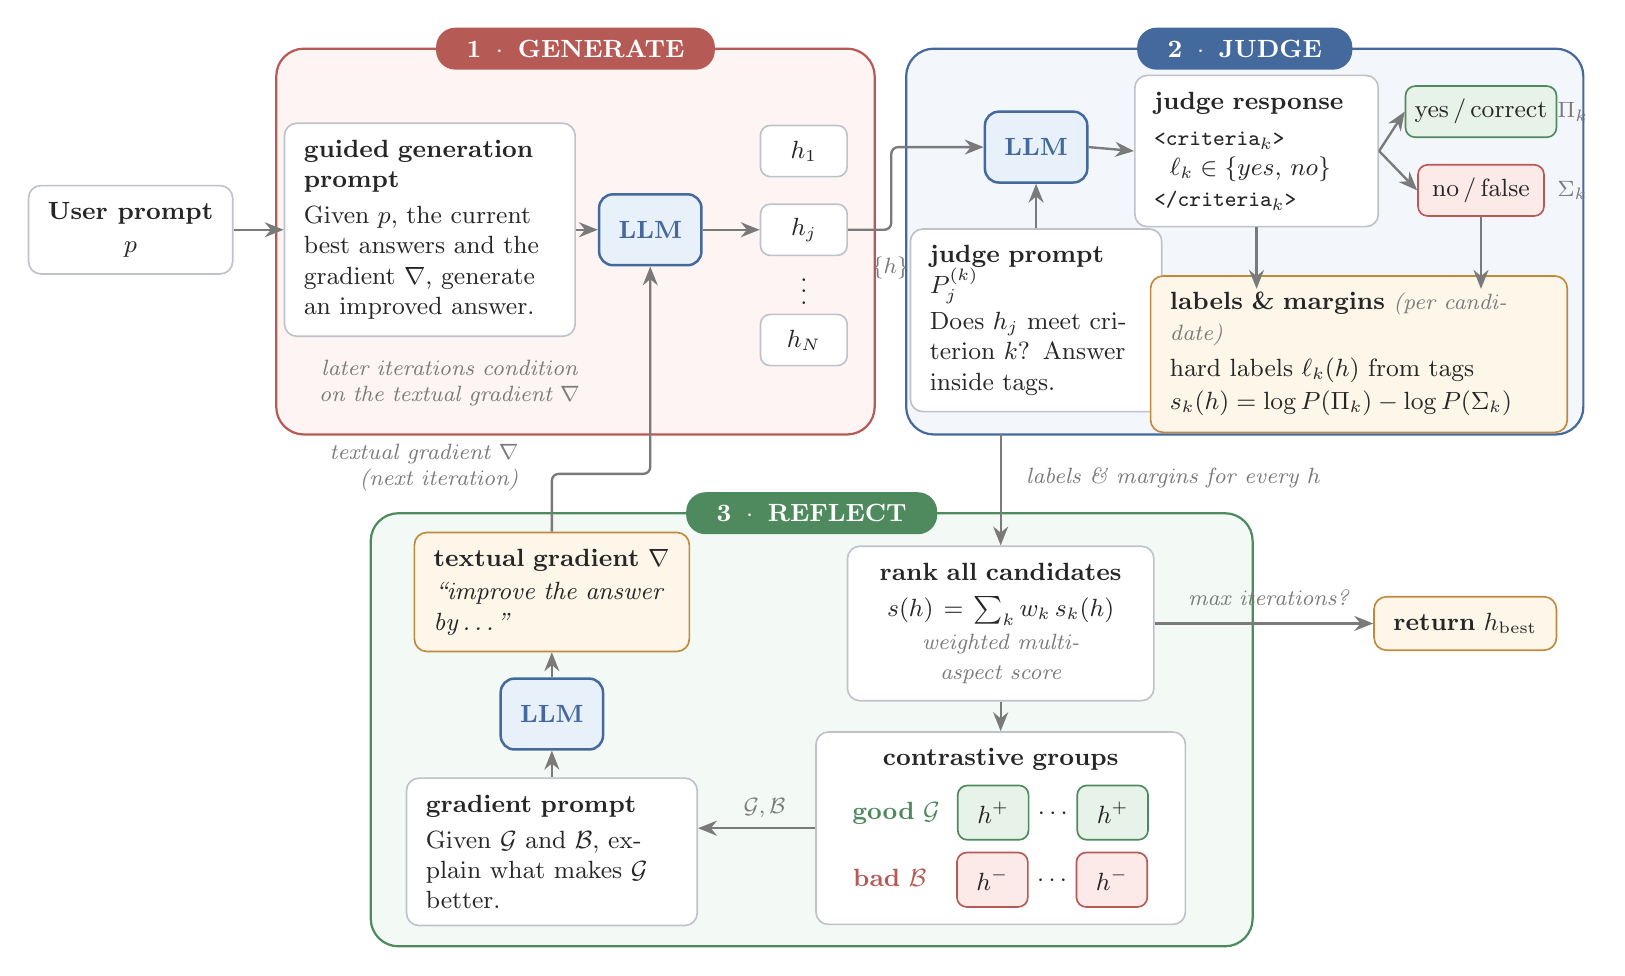
\begin{tikzpicture}[x=1cm,y=1cm]

% ================= PANELS (fixed rectangles) =================
\begin{scope}[on background layer]
  \draw[fill=genF, draw=genA, line width=0.8pt, rounded corners=10pt] (3.0,6.7) rectangle (10.6,11.6);
  \draw[fill=judF, draw=judA, line width=0.8pt, rounded corners=10pt] (11.0,6.7) rectangle (19.6,11.6);
  \draw[fill=refF, draw=refA, line width=0.8pt, rounded corners=10pt] (4.2,0.2) rectangle (15.4,5.7);
\end{scope}
\node[hdr, fill=genA] at (6.8,11.6)  {1\,\ $\cdot$\ \,GENERATE};
\node[hdr, fill=judA] at (15.3,11.6) {2\,\ $\cdot$\ \,JUDGE};
\node[hdr, fill=refA] at (9.8,5.7)   {3\,\ $\cdot$\ \,REFLECT};

% ================= USER =================
\node[card, align=center] (user) at (1.15,9.3) {\hd{User prompt}\\[1pt]$p$};

% ================= GENERATE =================
\node[card, text width=32mm] (genprompt) at (4.95,9.3)
  {\hd{guided generation prompt}\\[2pt]
   Given $p$, the current best answers and the gradient $\nabla$, generate an improved answer.};
\node[llm] (genllm) at (7.75,9.3) {LLM};
\node[hbox] (h1) at (9.7,10.3) {$h_1$};
\node[hbox] (hj) at (9.7,9.3)  {$h_j$};
\node[hbox] (hN) at (9.7,7.9)  {$h_N$};
\node at (9.7,8.62) {$\vdots$};
\node[note, text width=40mm] at (5.2,7.35)
  {later iterations condition\\ on the textual gradient $\nabla$};

% ================= JUDGE =================
\node[card, text width=27mm] (judprompt) at (12.65,8.15)
  {\hd{judge prompt} $P^{(k)}_j$\\[2pt]
   Does $h_j$ meet criterion $k$? Answer inside tags.};
\node[llm] (judllm) at (12.65,10.35) {LLM};
\node[card, text width=26mm] (judresp) at (15.45,10.3)
  {\hd{judge response}\\[2pt]
   {\ttfamily\footnotesize <criteria$_k$>}\\
   \hspace*{2mm}$\ell_k \in \{\text{yes},\,\text{no}\}$\\
   {\ttfamily\footnotesize </criteria$_k$>}};
\node[chip, fill=posF, draw=refA] (yes) at (18.3,10.8) {yes\,/\,correct};
\node[chip, fill=negF, draw=genA] (no)  at (18.3,9.8)  {no\,/\,false};
\node[note, anchor=west] at (19.15,10.8) {$\Pi_k$};
\node[note, anchor=west] at (19.15,9.8) {$\Sigma_k$};
\node[card, text width=48mm, fill=ambF, draw=ambA] (outs) at (16.75,7.72)
  {\hd{labels \& margins}\ {\itshape\footnotesize\color{arw}(per candidate)}\\[2pt]
   hard labels $\ell_k(h)$ from tags\\[1pt]
   $s_k(h)=\log P(\Pi_k)-\log P(\Sigma_k)$};

% ================= REFLECT =================
\node[card, text width=34mm, align=center] (rank) at (12.2,4.3)
  {\hd{rank all candidates}\\[2pt]
   $s(h)=\sum_k w_k\, s_k(h)$\\[1pt]
   {\itshape\footnotesize\color{arw} weighted multi-aspect score}};
\node[card, text width=42mm, align=center] (groups) at (12.2,1.7)
  {\hd{contrastive groups}\\[4pt]
   {\color{refA}\bfseries good $\mathcal{G}$}\ \
   \tikz[baseline=-0.6ex]{\node[gchip,fill=posF,draw=refA]{$h^{+}$};}\
   $\cdots$\
   \tikz[baseline=-0.6ex]{\node[gchip,fill=posF,draw=refA]{$h^{+}$};}\\[3pt]
   {\color{genA}\bfseries bad $\mathcal{B}$}\ \ \,
   \tikz[baseline=-0.6ex]{\node[gchip,fill=negF,draw=genA]{$h^{-}$};}\
   $\cdots$\
   \tikz[baseline=-0.6ex]{\node[gchip,fill=negF,draw=genA]{$h^{-}$};}};
\node[card, text width=32mm] (gcprompt) at (6.5,1.4)
  {\hd{gradient prompt}\\[2pt]
   Given $\mathcal{G}$ and $\mathcal{B}$, explain what makes $\mathcal{G}$ better.};
\node[llm] (refllm) at (6.5,3.15) {LLM};
\node[card, text width=30mm, fill=ambF, draw=ambA] (grad) at (6.5,4.7)
  {\hd{textual gradient} $\nabla$\\[1pt]
   {\itshape``improve the answer by\,\dots''}};

% ================= RETURN =================
\node[card, fill=ambF, draw=ambA, align=center] (ret) at (18.1,4.3)
  {\hd{return} $h_{\mathrm{best}}$};

% ================= ARROWS =================
\draw[flow] (user.east) -- (genprompt.west);
\draw[flow] (genprompt.east) -- (genllm.west);
\draw[flow] (genllm.east) -- (hj.west);
\draw[flow] (hj.east) -- ++(0.55,0) |- (judllm.west);
\node[note] at (10.8,8.82) {$\{h\}$};
\draw[flow] (judprompt.north) -- (judllm.south);
\draw[flow] (judllm.east) -- (judresp.west);
\draw[flow] (judresp.east) -- (yes.west);
\draw[flow] (judresp.east) -- (no.west);
\draw[flow] (judresp.south) -- (15.45,8.55);
\draw[flow] (no.south) -- (18.3,8.55);
\draw[flow] (12.2,6.7) -- (rank.north);
\node[note, anchor=west] at (12.4,6.15) {labels \& margins for every $h$};
\draw[flow] (rank.south) -- (groups.north);
\draw[flow] (groups.west) -- (gcprompt.east |- groups.west);
\node[note] at (9.2,1.95) {$\mathcal{G},\mathcal{B}$};
\draw[flow] (gcprompt.north) -- (refllm.south);
\draw[flow] (refllm.north) -- (grad.south);
\draw[flow] (grad.north) -- (6.5,6.2) -- (7.75,6.2) -- (genllm.south);
\node[note, anchor=east, align=right] at (6.2,6.28) {textual gradient $\nabla$\\ (next iteration)};
\draw[flow] (rank.east) -- (ret.west);
\node[note] at (15.6,4.62) {max iterations?};

\end{tikzpicture}
\end{document}
